\subsection{Mounting a crystal on the diffractometer}

	\begin{figure*}[t]
		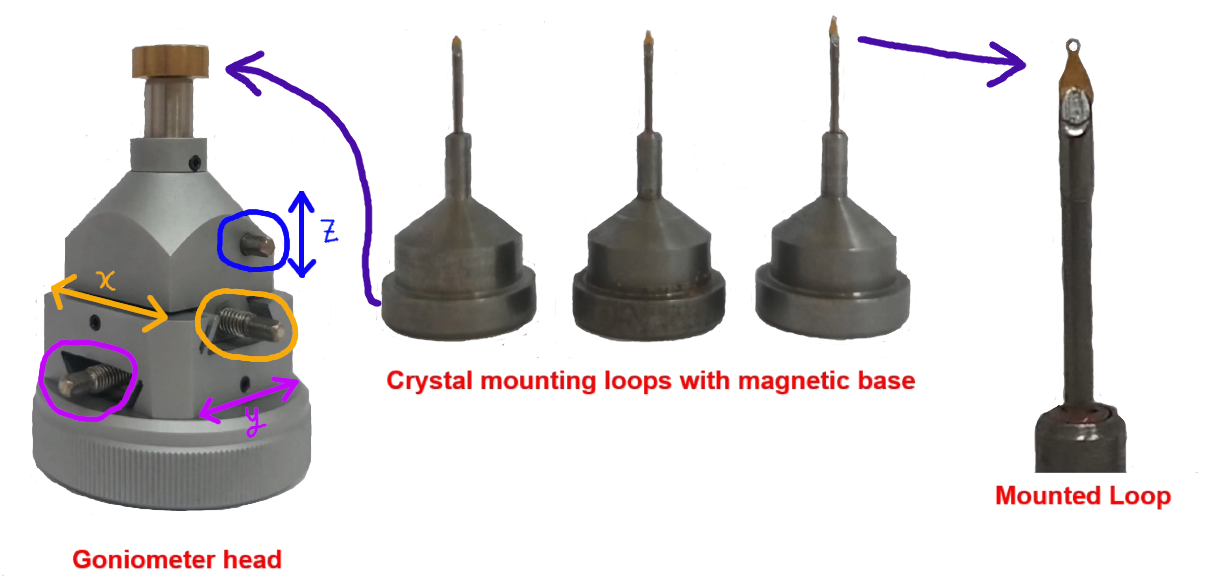
\includegraphics[scale=0.5]{goniometer1.png}
		\caption{\label{fig:goniometer}The goniometer head, mounting loop with the mounting base. Image courtesy:~\cite{Chowdhury2022}.}
	\end{figure*}

	In fig.~\ref{fig:goniometer}, a goniometer head is shown. This head is mounted on the goniometer of the diffractometer. The top of the goniometer head is a magnetic base which allows the mounting loops to be held in place. To align the crystal in the X-ray beam, the goniometer head has three screws that allow movement in the three Cartesian directions. These screws and their respective directions have been demarcated in the figure.

		The tip of the mounting metal pin has a small polymer loop. The crystal is mounted on this loop using some thick oil, which keeps the crystal in place by its surface tension. These loops are available in various diameters, generally in the range $0.05-0.5~\si{mm}.$

		Nylon loops are also available, in which the loop is made by a nylon thread, which is then twisted several times and then glued to a pin. The pin is attached to a brush, which can be directly mounted on the goniometer head and placed in the X-ray beam.